%% LyX 2.1.4 created this file.  For more info, see http://www.lyx.org/.
%% Do not edit unless you really know what you are doing.
\documentclass[english]{article}
\usepackage{mathptmx}
\usepackage{helvet}
\usepackage{courier}
\usepackage[T1]{fontenc}
\usepackage[latin9]{inputenc}
\usepackage{geometry}
\geometry{verbose,tmargin=1in,bmargin=1in,lmargin=1in,rmargin=1in,headheight=0in,headsep=0in}
\pagestyle{empty}
\usepackage{babel}
\usepackage{graphicx}
\usepackage[unicode=true]
 {hyperref}

\makeatletter

%%%%%%%%%%%%%%%%%%%%%%%%%%%%%% LyX specific LaTeX commands.
%% Because html converters don't know tabularnewline
\providecommand{\tabularnewline}{\\}

%%%%%%%%%%%%%%%%%%%%%%%%%%%%%% User specified LaTeX commands.
\date{}

\makeatother

\begin{document}
\begin{center}
\textbf{\large{}CSCE 221 Assignment 6 Cover Page}\\
\bigskip{}

\par\end{center}

First Name~~~~~~~~~~~~Chris~~~~~~~~~~Last Name
~~~~~~~Comeaux~~~~~~~~~UIN~~~~622006681~~~~~~~~~~\bigskip{}


User Name ~~~~~~~~cmc236~~~~~~~~~~~~~~~~~~~~~E-mail
address~~~~~~~cmc236@tamu.edu~~~~~~~~~~~~~~~~~~~~~~~\medskip{}


Please list all sources in the table below including web pages which
you used to solve or implement the current homework. If you fail to
cite sources you can get a lower number of points or even zero, read
more on Aggie Honor System Office website: \texttt{\href{http://aggiehonor.tamu.edu/}{http://aggiehonor.tamu.edu/}}\medskip{}
\medskip{}


\noindent \begin{flushleft}
\begin{tabular}{|c|c|c|}
\hline 
Type of sources  & ~~~~~~~~~~~~~~~~~~~~~~~ & ~~~~~~~~~~~~~~~~~~~~~~~~\tabularnewline
 &  & \tabularnewline
\hline 
People & Peer Teacher & Dr. Teresa Leyk\tabularnewline
 &  & \tabularnewline
\hline 
Web pages (provide URL)  & http://www.cplusplus.com/forum/beginner/89137/ & http://programmers.stackexchange.com/\tabularnewline
 & http://www.cplusplus.com/reference/list/list/erase/ & \tabularnewline
\hline 
Printed  &  & \tabularnewline
 &  & \tabularnewline
\hline 
Other Sources  &  & \tabularnewline
 &  & \tabularnewline
\hline 
\end{tabular}
\par\end{flushleft}

\medskip{}
\medskip{}


\noindent I certify that I have listed all the sources that I used
to develop the solutions/codes to the submitted work.

\noindent \emph{On my honor as an Aggie, I have neither given nor
received any unauthorized help on this academic work}.

\bigskip{}
\bigskip{}


\begin{tabular}{cccccc}
Your Name  & Chris &  & Comeaux & Date  & 4/24/2016\tabularnewline
\end{tabular}

\pagebreak{}


\section*{Assignment 6 Description}

In programming Assignment 6, students had to represent any directed
graph as a directed acyclic graph (DAG). To to this, students had
to extract the strongly connected components of the graph and represent
them as a single vertex. In the first part of the program, students
had to read in an adjacency list, create a graph from the list, and
print the graph to the screen (as an adjacency list). In the second
part, students had to run a depth first search on the graph to find
the search order, create a transpose of the graph, and run the depth
first search on the transpose. Running the depth first search on the
transpose will return the strongly connected components. From there,
students had to use the strongly connected components found in the
last step and create the final acyclic graph. 


\section*{Implementation}

To implement the notion of a graph I used a STL vector of vertices.
Each vertex comprised of an edgeList and a label. The edgeList was
a STL list of edges. An edge contained a starting label, end label,
a weight, and a visited bit. The starting label represented the starting
node of a directed edge and the end label represented the ending node
of a directed edge. To display the graph to the screen, I outputted
the graph as an adjacency list in the displayGraph() member function
of the Graph class. To transpose the graph (reverseGraph(Graph\& T)),
I visited every edge in every vertices' edge list, created a new edge
in the corresponding transpose graph's vertices edgeList, and reversed
the start and finish label. The depth first search was implemented
through two functions: getDFSOrder and getDFSOrder. These functions
utilized a stack and two vectors. One vector held the visited nodes
while the other vector held the order of nodes starting from the lowest
end time stamp to the highest end time stamp. The stack was used to
keep track of the nodes in the current path. To create the final DAG,
makeSCG(Graph graph, vector<int> order) was called on the transpose
graph. Like the two functions listed above, makeSCG(Graph graph, vector<int>
order), utilized 2 vectors and one stack implemented in the same manor.
However, this function had an additional vector of vectors of ints.
The inner vector each represented one strongly connected component.
This vector of vector of ints was then used to extract the strongly
connected components from the original graph and create a new graph
with the vertices. Finally, the function deleted all edges that did
not belong in the DAG, checked for any loops, and displayed the graph
to the screen.


\section*{C++ Features Used}

I did not use any aspects of generic programming in programming assignment
6. However, I did use some object oriented programming features such
as abstraction. I created 3 objects, a Graph object, a Vertex object,
and a Edge object. The implementation of Edge was hidden behind the
Vertex object and the implementation of Vertex was hidden behind the
Graph object. Each object knew about the class below it but not above
it. For example, the Graph class knew what a Vertex and Edge was,
the Vertex class knew what a Edge was but did not know anything about
the Graph class, and the Edge class did not know anything about the
Vertex or Graph classes. Another C++ feature was that I used 3 standard
library containers in my implementation: stack, vector, and list. 


\section*{Assumptions on Input Data}

There were a few assumptions made on the input data. The first assumption
was that the input was in the form of an adjacency list. Furthermore,
this adjacency list had to be terminated by a -1 and on a separate
line. Finally, an assumption was made that each number in the list
was separated by a space. A visual representation of these assumptions
would be: \# \# \# \# -1, where \# represents any number and is not
limited to the number of \# listed. 


\section*{Testing}

\begin{flushleft}
I used three test cases to test my program listed below. NOTE: the
adjacency list listed under GRAPH is identical to the input data.
\begin{minipage}[t]{1\columnwidth}%
\textbf{Test1:\textbf{$\newline$}}

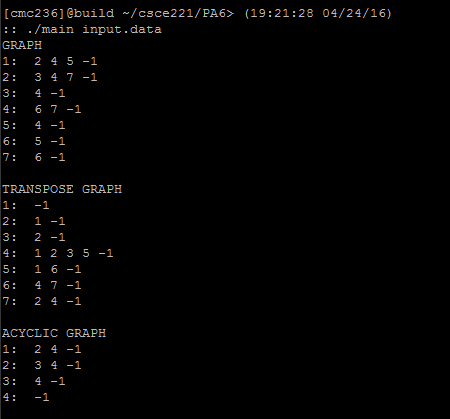
\includegraphics{Test1}

\textbf{Test 2: \textbf{$\newline$}}

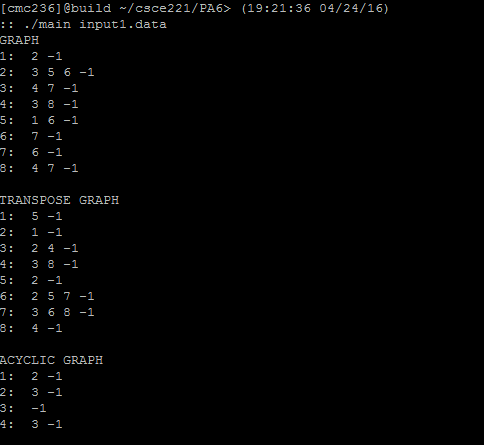
\includegraphics{Test2}%
\end{minipage}
\par\end{flushleft}

\newpage{}%
\begin{minipage}[t]{1\columnwidth}%
\begin{flushleft}
\textbf{Test 3:\textbf{$\newline$}}
\par\end{flushleft}

\begin{flushleft}
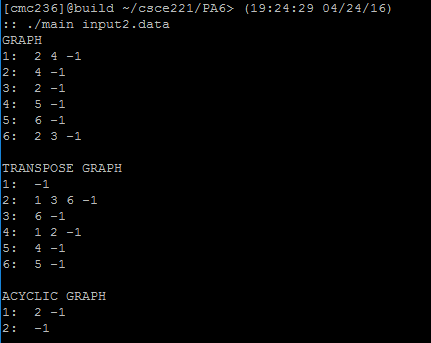
\includegraphics{Test3}
\par\end{flushleft}%
\end{minipage}


\section*{Running Time Functions}

\begin{minipage}[t]{1\columnwidth}%
\textbf{GRAPH:}

\textbf{buildGraph:} O($n*m$) where n is the number of lines in the
file and m is the number of characters in each line. This is because
the this function reads in one line at a time then does work on each
character in each line.

\textbf{displayGraph: }O($n*m$). This is because this function loops
through every edge and vertex in the graph. n is the number of vertices
and m is the number of edges.

\textbf{reverseGraph: }O(n{*}m) Like the function above, this function
loops through every edge and every vertex. n is the number of vertices
and m is the number of edges.

\textbf{findLabel: }O(n) where n is the number of vertices. This function
loops through each every vertex and return the index of the vertex
with the label that was passed to it.

\textbf{getDFSOrder: }O(1) This function is constant because it simply
initializes the depth first search. It first finds the index of the
first vertex, add that vertex to the the visited vector and vertex
stack and then calls vertex traversal.

\textbf{vertexTraversal: }O(n) This function is recursive and continues
to call itself as long as all vertices have not been visited. Since
it visits all vertices it is O(n) where n is the number of vertices.

\textbf{makeSCG:} O(n{*}m) This function, like the other listed above,
visits every vertex and every edge in the output graph. even though
it has many loops, its can be bounded by O(n{*}m) where n is the number
of vertices in the graph and m is the nuber of edges in the graph

\textbf{VERTEX}

\textbf{reverseEdge: }O(n) where n is the number of edges in the edge
list. This is because this function loops though every node in the
edgeList and reverses the edge

\textbf{isVisited: }O(n) where n is the number of vertices in the
visited vector. This function compares the passed value to every number
in the vector too see if has been visited or not.

\textbf{isVertex: }O(n) where n is the number of vertices in the graph
call on. This vertex compares the passed label to every label in the
vertices vector to see if there is a corresponding vertex with that
label.

\textbf{isLoop: }O(n{*}m) where n is the number of vertices in the
graph and m is the number of edges in the graph. This function goes
through every vertex's edges and sees if there is any type of loop. %
\end{minipage}


\section*{Real Life Application }

One application that this program can be used is when calculating
the maximum execution time of a set. To do this we need to have a
DAG of the set in memory. Since my program can be used to create a
DAG from any directed graph, you could pass the original graph to
my program, extract the DAG and then pass it to another algorithm
that calculates the maximum execution time of the set. 


\section*{Conclusion}

Programming assignment 6 taught students about graphs and graph traversals,
especially depth first search. To complete the this assignment students
had to understand graphs enough to represent a graph in c++ and then
write a depth first search to traverse the graph. Furthermore, the
students had to understand what strongly connected components were
and how to recognize them in graphs to create a DAG from any directed
graph. 
\end{document}
